%------------------------------------------------------------------------------------------------------------
\section{Inference engine} \label{sec:InferenceEngine}
%------------------------------------------------------------------------------------------------------------

In this section we provide an overview of the current implementation status of the AMIDST toolbox related to inference algorithms. Figure \ref{Figure:InferenceEngine} illustrates the main core components of the toolbox. The color coding in the figure summarizes the implementation status: blue bodes represent software components that have been implemented in the AMIDST toolbox and green boxes represent components that are part of the software design specification but which have not yet been implemented.

\vspace{-0.1in}

\begin{figure}[ht!]
\begin{center}
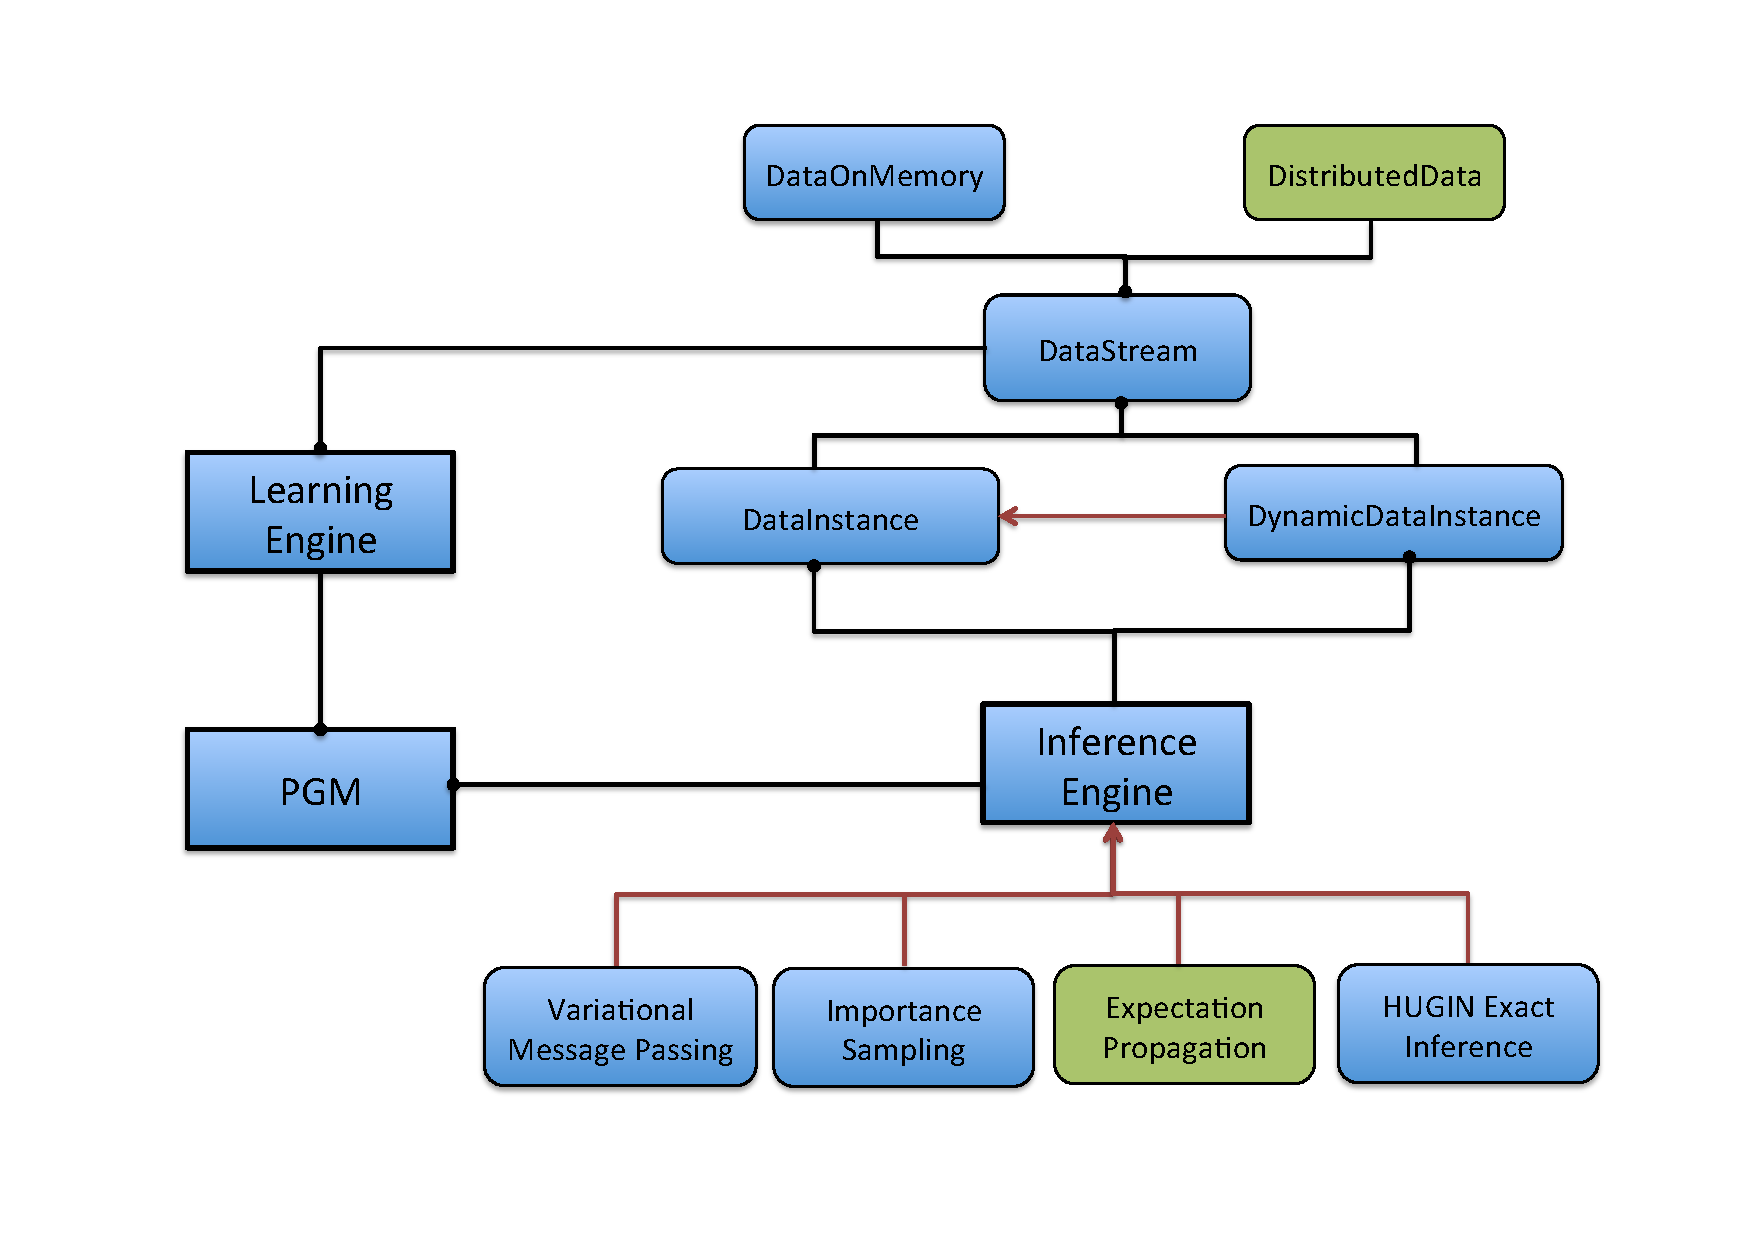
\includegraphics[width=\linewidth]{./figures/InferenceEngine}
\vspace{-0.5in}
\caption{\label{Figure:InferenceEngine} Illustration of AMIDST toolbox main core components. Nomenclature: The boxes in the
      figure represent software components (sets, possibly singletons, of classes), a rounded-arc going from $X$ to $Y$ indicates that $Y$ 'uses/references' $X$, and an arc with an arrow from $X$ to $Y$ implies inheritance.}
\end{center}
\end{figure}

Note that some of the core components of the AMIDST toolbox, shown in Figure \ref{Figure:InferenceEngine}, have already been introduced in the previous deliverables. Deliverable 4.1 \cite{Deliverable4.1} described the status of the software development in respect to the \comp{Learning Engine} component including BN structural and parameter learning as well as the parallelization of structural learning using parallel TAN and PC implementations. Deliverable 2.3 \cite{Deliverable2.3} provided more details about the data structures related to the \comp{PGM} component and the different considered data source management functionalities, namely, \comp{DataOnMemory}, \comp{DataOnDisk}, \comp{DistributedData}, \comp{DataStream}, \comp{DataInstance}, and \comp{DynamicDataInstance}.

In this section, we focus on the \comp{Inference Engine} component for which we will present in what follows the considered derived components, namely, \comp{Variational Message Passing}, \comp{Importance Sampling}, \comp{Expectation Propagation}, and \comp{HUGIN Exact Inference}.


%------------------------------------------------------------------------------------------------------------
\subsection{Variational Message Passing (VMP)} \label{VMP}
%------------------------------------------------------------------------------------------------------------

A general architecture for supporting variational message passing (\comp{VMP}) in graphical models is presented in \cite{Bishop2005}, highlighting how distributions that are conjugate-exponential families \cite{Attias2000,Beal2003,Bishop2005} can be utilised to efficiently represent the messages by the expected natural statistics. A similar scheme can also be deployed for expectation propagation, but there relying on a transformation between the exponential family representation?s expected sufficient statistics and the distribution?s moments.


%------------------------------------------------------------------------------------------------------------
\subsection{Importance Sampling (IS)} \label{IS}
%------------------------------------------------------------------------------------------------------------

Importance Sampling (IS) \cite{Yuan2007} is based on the Hybrid Loopy Belief propagation.


%------------------------------------------------------------------------------------------------------------
\subsection{Expectation Propagation (EP)} \label{EP}
%------------------------------------------------------------------------------------------------------------

Expectation propagation (\comp{EP}) \cite{Minka2001} presents a similar approximation scheme as VMP, but it rely more on a transformation between the exponential family representation's expected sufficient statistics and the distribution's moments.


%------------------------------------------------------------------------------------------------------------
\subsection{HUGIN Exact Inference} \label{HuginInference}
%------------------------------------------------------------------------------------------------------------

